\begin{section}{Problem 4}
    \begin{problem}{4}
        Load the following .mat matrix that appears on the assignment page:
        \begin{verbatim}
    load powerMatrix;
        \end{verbatim}
        If you hit {\tt whos} you should be seeing a matrix called $A$, of size $100 \times 100$. To validate any of your results below, you may run the {\sc {Matlab}} command {\tt eig}, as long as you understand that in typical eigenvalue computations (in a potentially more challenging computational environment) we generally do not have the luxury of running  {\tt eig} to check ourselves. 
        \begin{enumerate}[(a)]
            \item Apply the power method. Terminate the iteration once the iterates satisfy $$ \lambda_1^{(k)}-\lambda_1^{(k-1)}| < 10^{-4}.$$ Your program should print out the value of the final iterate and a graph of the absolute errors: $| \lambda_1^{(k)}-\lambda_{\max}|$. For better visualization, use {\tt semilogy}  for your graphs when necessary. As an initial guess for the eigenvector use a vector produced by the \textsc{Matlab} command {\tt randn}. (When you repeat your experiments, the number of iterations may slightly vary due to the random initial guess.)
            \item Repeat your computations with the {\em inverse} power iteration, with a shift $\alpha=4$, and produce the same graph as you did for the power method.
            \item Discuss the differences between the performance of the power and the inverse power methods in terms of the cost of single iterations and t overall computational cost.
            \item Suppose now that we know that $A$ has an eigenvalue close to 3 and we are interested to compute it to six correct decimal digits. Suggest an efficient procedure for doing so. Implement your suggested algorithm and compute the eigenvalue.
        \end{enumerate}
    \end{problem}

    \newpage

    \begin{solution}{a}
        \begin{mdframed}
            \footnotesize
            \textbf{File: {\tt DevamSisodraker\_4a.m}}
            \inputminted{matlab}{DevamSisodraker_4a.m}
            \normalfont
        \end{mdframed}
        
        \continued
        
        \begin{mdframed}
            \footnotesize
            \textbf{File: {\tt DevamSisodraker\_4a\_out.txt}}
            \inputminted{matlab}{DevamSisodraker_4a_out.txt}
            \normalfont
        \end{mdframed}

        \continued

        \begin{mdframed}
            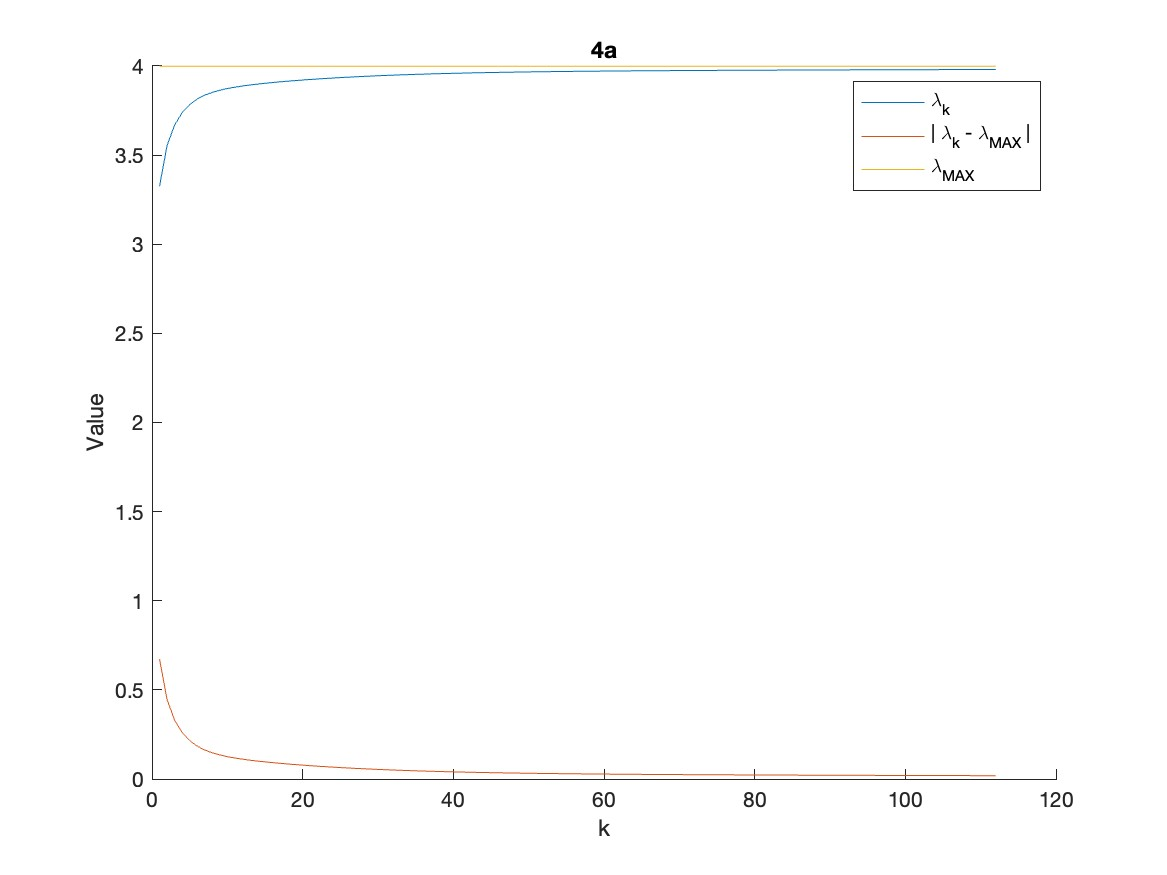
\includegraphics[scale=0.33]{DevamSisodraker_4a.jpg}
        \end{mdframed}
    \end{solution}

    \begin{solution}{b}
        \begin{mdframed}
            \footnotesize
            \textbf{File: {\tt DevamSisodraker\_4b.m}}
            \inputminted{matlab}{DevamSisodraker_4b.m}
            \normalfont
        \end{mdframed}
        
        \continued
        
        \begin{mdframed}
            \footnotesize
            \textbf{File: {\tt DevamSisodraker\_4b\_out.txt}}
            \inputminted{matlab}{DevamSisodraker_4b_out.txt}
            \normalfont
        \end{mdframed}

        \continued

        \begin{mdframed}
            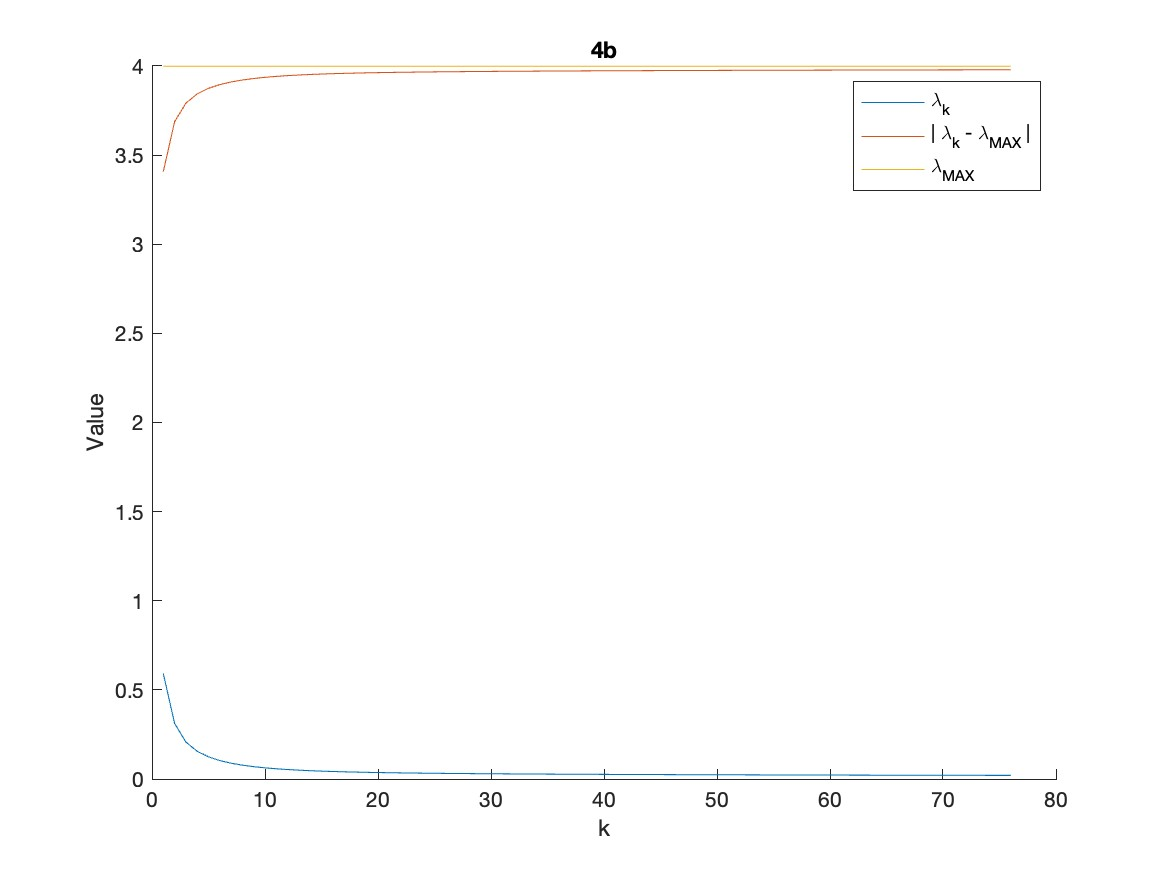
\includegraphics[scale=0.33]{DevamSisodraker_4b.jpg}
        \end{mdframed}
    \end{solution}

    \newpage
    
    \begin{solution}{c}
        thing
    \end{solution}
\end{section}